
\begin{lemma}
The points of intersection of line \\L:$\vec{x}=\vec{q}+\mu \vec{m}$ with the conic 
\begin{align}
\vec{x}^\top\vec{V}\vec{x}+2\vec{u}^\top\vec{x}+f=0
\end{align}
are given by 
\begin{align}  \vec{x_{i}}=\vec{q}+\mu_{i}\vec{m}
\end{align}
where 
\begin{multline}
    \mu_i=\frac{1}{\vec{m}^\top\vec{V}\vec{m}}-\vec{m}^\top\brak{\vec{V}\vec{q}+\vec{u}}\\ \pm\sqrt{[\vec{m}^\top(\vec{V}\vec{q}+\vec{u})]-(\vec{q}^\top\vec{V}\vec{q}+2\vec{u}^\top\vec{q}+\f)(\vec{m}^\top\vec{V}\vec{m})} 
\end{multline}

\end{lemma}
The equation of line $\myvec{1 & -\sqrt{3}}\vec{x}=0$ can also be expressed as $\vec{x}=\mu \myvec{1 \\ \frac{1}{\sqrt{3}}}$.\\
The matrix parameters of the circle $\vec{x}^\top\vec{x}=4$ are
\begin{align}
    \vec{V}&=\myvec{1&0\\0&1}\\
    \vec{u}&=\myvec{0\\0}\\
    f &= -4
\end{align}

The points of intersection of the line $\vec{x}=\mu \myvec{1 \\ \frac{1}{\sqrt{3}}}$ and the circle $\vec{x}^\top\vec{x}=4$ are 
\begin{align}
    \vec{x_i}&=\vec{q}+\mu_i\vec{m}\\
             &=\mu_i\myvec{1\\ \frac{1}{\sqrt{3}}}
\end{align}
where 
\begin{align}
    \mu_i = \pm\sqrt{3}
\end{align}
As the required point of intersection lies in first quadrant we have $\mu_i>0$
\begin{align}
    \implies \vec{A}=\sqrt{3}\myvec{1\\ \frac{1}{\sqrt{3}}}=\myvec{\sqrt{3}\\1}
\end{align}
The points of intersection of the line $\vec{x}=\mu\myvec{1\\0}$ and the circle $\vec{x}^\top\vec{x}=4$ are 
\begin{align}
    \vec{X_j}&=\vec{q}+\mu_j\vec{m}\\
             &=\mu_j\myvec{1\\0}
\end{align}
where
\begin{align}
    \mu_j = \pm 2
\end{align}
As the required point of intersection lies in first quadrant we have $\mu_j>0$
\begin{align}
    \implies \vec{B}&=2\myvec{1\\0}=\myvec{2\\0}
\end{align}
The angle($\theta$) of the sector AOB is 
\begin{align}
    \cos{\theta}&=\frac{\vec{A}^{\top}\vec{B}}{\norm{\vec{A}}\norm{\vec{B}}}\\
    &=\frac{2\sqrt{3}}{2\times 2}\\
    &=\frac{\sqrt{3}}{2}\\
    \implies \theta &= 30^{\degree}
\end{align}
\begin{align}
    \text{Area of the sector}&=\brak{\frac{\theta}{360^{\degree}}}\pi r^2\\
    &= \frac{\pi}{3}
\end{align}

\begin{figure}[!h]
 \centering
 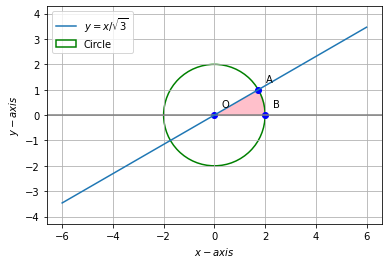
\includegraphics[width=\columnwidth]{solutions/oct/2/5/figs/fig.png}
 \caption{Reference plot}
 \label{oct/2/5/plot}
\end{figure}
